%\documentclass[manuscript]{geophysics}
%\usepackage[nomarkers]{endfloat}
% For a two-column format that looks like the final product, uncomment bellow
% and comment the two lines above
\documentclass[paper,twocolumn,twoside]{geophysics}

\usepackage{graphicx}
\usepackage{amsmath}


\newcommand{\vect}[1]{\mathbf{#1}}
\newcommand{\mat}[1]{\mathbf{#1}}
\newcommand{\comp}[1]{#1^{\alpha\beta}}
\newcommand{\norm}[1]{\left|\left|#1\right|\right|}

\begin{document}

\title{
    Tesseroids:
    command-line tools for
    gravity field forward modeling
    in spherical coordinates
}

% manuscript number
\ms{}

\address{
    \footnotemark[1]
    Universidade do Estado do Rio de Janeiro, Rio de Janeiro, Brazil,
    e-mail: leouieda@gmail.com;\\
    \footnotemark[2]
    Observat\'orio Nacional, Rio de Janeiro, Brazil;
}

\author{Leonardo Uieda\footnotemark[1]\footnotemark[2],
        Vanderlei C. Oliveira Jr\footnotemark[2],
        and
        Val\'eria C. F. Barbosa\footnotemark[2]}

\lefthead{Uieda et al.}
\righthead{Gravity forward modeling with Tesseroids}


%%%%%%%%%%%%%%%%%%%%%%%%%%%%%%%%%%%%%%%%%%%%%%%%%%%%%%%%%%%%%%%%%%%%%%%%%%%%%%%%
\begin{abstract}
Lorem ipsum dolor sit amet, consectetur adipiscing elit. Nam eu dolor pretium,
egestas mauris sed, dapibus quam. Duis hendrerit mollis nunc a consequat. Nulla
et sem consectetur, interdum velit eget, aliquam ipsum. Praesent sagittis
tortor diam, sed ultrices magna ullamcorper vitae. Proin vitae orci augue.
Morbi dictum ligula gravida sem malesuada facilisis. Mauris nibh metus, cursus
eget imperdiet vitae, pretium at lorem. Praesent nisi mauris, pretium ut risus
fermentum, egestas tincidunt nibh. Mauris nulla orci, consequat eu pharetra
non, mattis ut urna. Mauris facilisis orci eros. Nam mattis non magna iaculis
consectetur. Morbi sodales dolor vitae felis sagittis, eget faucibus turpis
convallis. Nullam malesuada, mauris et ultricies rutrum, odio nulla gravida
nunc, ac volutpat eros lectus eget lacus. Integer venenatis velit vel justo
pellentesque, quis molestie sem vestibulum.
\end{abstract}

%%%%%%%%%%%%%%%%%%%%%%%%%%%%%%%%%%%%%%%%%%%%%%%%%%%%%%%%%%%%%%%%%%%%%%%%%%%%%%%%
\section{Introduction}

Citing articles in text \citet{Asgharzadeh2007} and with parenthesis
\citep{Braitenberg2011}.


%%%%%%%%%%%%%%%%%%%%%%%%%%%%%%%%%%%%%%%%%%%%%%%%%%%%%%%%%%%%%%%%%%%%%%%%%%%%%%%%
\section{Methodology}

The gravitational potential,
gravitational acceleration,
and Marussi (gravity gradient) tensor
caused by a homogeneous tesseroid
with density $\rho$
are \citep{Grombein2013}

\begin{equation}
    V(r,\phi,\lambda) = G \rho
        \int\limits_{\lambda_1}^{\lambda_2}
        \int\limits_{\phi_1}^{\phi_2}
        \int\limits_{r_1}^{r_2}
        \frac{1}{\ell} \kappa  dr' d\phi' d\lambda',
    \label{eq:tesspot}
\end{equation}
\begin{equation}
    g_{\alpha}(r,\phi,\lambda) = G \rho
        \int\limits_{\lambda_1}^{\lambda_2}
        \int\limits_{\phi_1}^{\phi_2}
        \int\limits_{r_1}^{r_2}
        \frac{\Delta_{\alpha}}{\ell^3} \kappa dr' d\phi' d\lambda'
        \ \ \ \alpha \in \{x,y,z\},
    \label{eq:tessgrav}
\end{equation}

\noindent
and

\begin{equation}
    g_{\alpha\beta}(r,\phi,\lambda) = G \rho
        \int\limits_{\lambda_1}^{\lambda_2}
        \int\limits_{\phi_1}^{\phi_2}
        \int\limits_{r_1}^{r_2}
        I_{\alpha\beta}
        dr' d\phi' d\lambda',
    \label{eq:tesstensor}
\end{equation}

\noindent
in which
$(\phi, \lambda, r)$ are
the latitude, longitude, and radius
coordinates of computation point P (Figure~\ref{fig:tesseroid}),
$\alpha,\beta \in \{x,y,z\}$
(the local coordinate system of point P),
and

\begin{eqnarray}
    I_{\alpha\beta} &=&
        \left(
            \frac{3\Delta_{\alpha} \Delta_{\beta}}{\ell^5} -
            \frac{\delta_{\alpha\beta}}{\ell^3}
        \right) \kappa, \\
    \Delta_x &=& r' K_{\phi} , \\
    \Delta_y &=& r' \cos \phi' \sin(\lambda' - \lambda) , \\
    \Delta_z &=& r' \cos \psi - r, \\
    \ell &=& \sqrt{r'^2 + r^2 - 2 r' r \cos \psi} , \\
    \cos\psi &=& \sin\phi\sin\phi' + \cos\phi\cos\phi'
                 \cos(\lambda' - \lambda) , \\
    K_{\phi} &=& \cos\phi\sin\phi' - \sin\phi\cos\phi'
                 \cos(\lambda' - \lambda), \\
    \kappa &=& {r'}^2 \cos \phi'.
\end{eqnarray}

\noindent
$\delta_{\alpha\beta}$ is the Kronecker delta,
i.e. $\delta_{\alpha\beta}=1$ if $\alpha=\beta$
and $\delta_{\alpha\beta}=0$ otherwise.

\begin{figure}
    \centering
    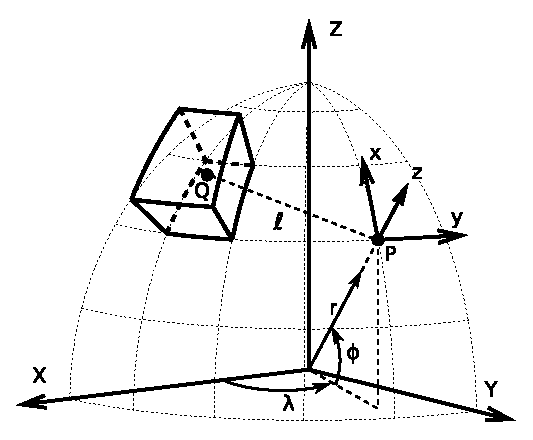
\includegraphics[width=\columnwidth]{figs/tesseroid}
    \caption{
        View of a tesseroid,
        the integration point $Q$,
        a geocentric coordinate system $(X, Y, Z)$,
        the computation $P$ and it's local coordinate system $(x, y, z)$.
        $r$, $\phi$, $\lambda$ are
        the radius, latitude, and longitude, respectively, of point $P$,
        and $\ell$ is the Cartesian distance between $P$ and $Q$.
    }
    \label{fig:tesseroid}
\end{figure}

The above integrals
have to be solved numerically
\citep{Wild-Pfeiffer2008}
and different approaches have been proposed.
\citet{Heck2007}
used a Taylor series expansion,
while \citet{Asgharzadeh2007}
used the Gauss-Legendre Quadrature (GLQ).
\citet{Wild-Pfeiffer2008} investigated
the use of both methods,
along with alternative mass elements,
and found the GLQ to be the most efficient method.
Therefore, we have opted to use
the 3D GLQ in our computations.

The Gauss-Legendre Quadrature
approximates the integral by
a weighted sum
\citep{Hildebrand1987},
e.g.

\begin{equation}
    \int\limits_a^b f(x) dx \approx
    \frac{b-a}{2}\sum\limits_{i=1}^N W_i f(x_i),
\end{equation}

\noindent
where the discretization points (nodes) $x_i$
are the roots of the $N$th order Legendre polynomial $P_N$
and the weights $W_i$ are \citep{Hildebrand1987}

\begin{equation}
    W_i = \frac{2}{(1 - x_i^2)(P'_N(x_i))^2}.
\end{equation}

The triple integrals in equations
\ref{eq:tesspot},
\ref{eq:tessgrav},
and
\ref{eq:tesstensor}
become

\begin{equation}
    V(r,\phi,\lambda) \approx
        A
        \sum\limits_{k=1}^{N^{\lambda}}
        \sum\limits_{j=1}^{N^{\phi}}
        \sum\limits_{i=1}^{N^r}
        W^r_i W^{\phi}_j W^{\lambda}_k
        \frac{1}{\ell} \kappa,
\end{equation}
\begin{equation}
    g_{\alpha}(r,\phi,\lambda) \approx
        A
        \sum\limits_{k=1}^{N^{\lambda}}
        \sum\limits_{j=1}^{N^{\phi}}
        \sum\limits_{i=1}^{N^r}
        W^r_i W^{\phi}_j W^{\lambda}_k
        \frac{\Delta_{\alpha}}{\ell^3} \kappa,
\end{equation}

\noindent
and

\begin{equation}
    g_{\alpha\beta}(r,\phi,\lambda) \approx
        A
        \sum\limits_{k=1}^{N^{\lambda}}
        \sum\limits_{j=1}^{N^{\phi}}
        \sum\limits_{i=1}^{N^r}
        W^r_i W^{\phi}_j W^{\lambda}_k
        I_{\alpha\beta},
\end{equation}

\noindent
where

\begin{equation}
    A = G \rho
    \frac{(\lambda_2 - \lambda_1)(\phi_2 - \phi_1)(r_2 - r_1)}{8},
\end{equation}

\noindent
$W_i^r$, $W_j^{\phi}$, and $W_k^{\lambda}$
are the weights
and $N^r$, $N^{\phi}$, and $N^{\lambda}$
are the number of nodes
for the radial, latitudinal, and longitudinal dimensions, respectively.

The accuracy of the numerical integration
using the GLQ
was investigated by \citet{Ku1977}
for the case of the right-rectangular prism.
\citet{Ku1977} found that the accuracy
depends on the ratio between
the average distance between GLQ nodes
and the distance to the observation point P.
As a rule-of-thumb,
\citet{Ku1977} suggests that
the distance between nodes
should not be greater than
the distance to point P.
\citet{Li2011} devised a scheme that
recursively subdivides the tesseroids
into smaller ones,
effectively decreasing the distance between nodes.
This scheme guarantees that
the rule-of-thumb is not violated.
Hence,
optimal accuracy of the numerical integration
is achieved automatically.



\begin{figure}
    \centering
    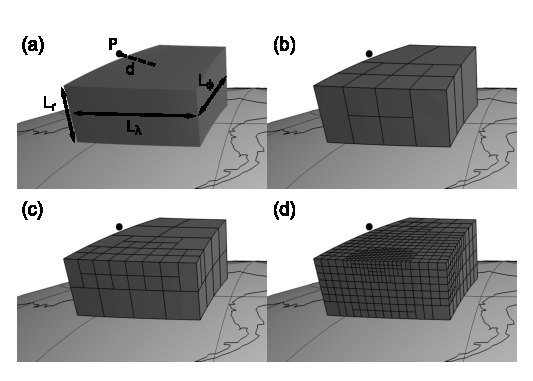
\includegraphics[width=\columnwidth]{figs/tesseroid-split}
    \caption{
        Adaptive discretization
        of the tesseroid shown in (a)
        for a computation point P
        using distance/size ratios of
        (b) 0.5, (c) 1, and (d) 2.
        $d$ is the distance between the tesseroid and P.
    }
    \label{fig:split}
\end{figure}


\subsection{Software implementation}

Lorem ipsum dolor sit amet, consectetur adipiscing elit. Nam eu dolor pretium,

\citet{Barrera-Figueroa2006}.

\subsection{Comparison with a spherical half-shell}


The potential of a spherical half-shell is

\begin{equation}
    V(r) = 2\pi G \rho \left[ \dfrac{l^3 + {r'}^3}{3r} - 0.5 {r'}^2 \right]
           \Biggr \rvert_{r'=r_1}^{r'=r_2}
    \label{eq:halfshell-pot}
\end{equation}

\noindent
where $\rho$ is the density,
$l = \sqrt{r^2 + {r'}^2}$,
$r$ is the radial coordinate of the observation point,
and
$r_1$ and $r_2$ are the bottom and top of the spherical shell,
respectively.

\begin{figure}
    \centering
    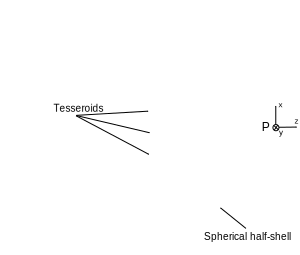
\includegraphics[width=\columnwidth]{figs/spherical-shell}
    \caption{This is a figure caption.}
    \label{fig:shell}
\end{figure}

This is a reference to Figure~\ref{fig:shell}.

The $g_z$ component of the gravitational attraction for this shell is the
radial derivative of the potential.

The sign should be inverted because our convention is that z points down
(toward the center of the Earth)

\begin{equation}
    g_z(r) = -\dfrac{\partial V}{\partial r} = 2\pi G \rho \left[ \dfrac{l^3 +
            {r'}^3}{3r^2} - l \right] \Biggr \rvert_{r'=r_1}^{r'=r_2}
    \label{eq:halfshell-gz}
\end{equation}

The gravity gradient tensor are the second derivatives of $V$:

\begin{equation}
    g_{xx}(r) = g_{yy}(r) = -\dfrac{1}{2} g_{zz}
\end{equation}

\begin{equation}
    g_{xy}(r) = g_{xz}(r) = g_{yz}(r) = 0
\end{equation}

\begin{equation}
    g_{zz}(r) = 2\pi G \rho \left[ 2\dfrac{l^3 + {r'}^3}{3r^3} - \dfrac{l}{r} +
    \dfrac{r}{l} \right] \Biggr \rvert_{r'=r_1}^{r'=r_2}
\end{equation}



%%%%%%%%%%%%%%%%%%%%%%%%%%%%%%%%%%%%%%%%%%%%%%%%%%%%%%%%%%%%%%%%%%%%%%%%%%%%%%%%
\section{Results}

%\begin{figure}
    %\centering
    %\subfigure[]{
        %\includegraphics[width=0.4\textwidth]{figs/sub1.png}\label{fig:sub1}}
    %\subfigure[]{
        %\includegraphics[width=0.4\textwidth]{figs/sub2.png}\label{fig:sub2}}
  %\caption{This is a figure caption.}
  %\label{fig:composite}
%\end{figure}

%This Figure \ref{fig:composite} is made up of Figure \ref{fig:sub1} and
%\ref{fig:sub2}.

\begin{figure}
    \centering
    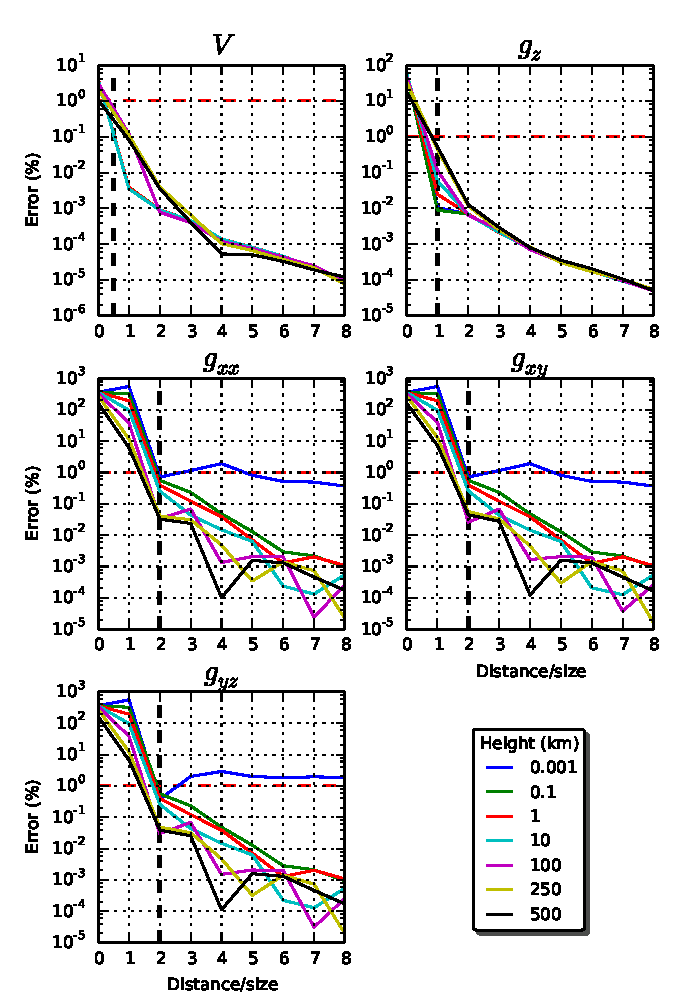
\includegraphics[width=\columnwidth]{figs/error-20deg}
    \caption{This is a figure caption.}
    \label{fig:error20}
\end{figure}

This is a reference to Figure \ref{fig:error20}.




%%%%%%%%%%%%%%%%%%%%%%%%%%%%%%%%%%%%%%%%%%%%%%%%%%%%%%%%%%%%%%%%%%%%%%%%%%%%%%%%
\section{Discussion}

%%%%%%%%%%%%%%%%%%%%%%%%%%%%%%%%%%%%%%%%%%%%%%%%%%%%%%%%%%%%%%%%%%%%%%%%%%%%%%%%
\section{Conclusions}

%%%%%%%%%%%%%%%%%%%%%%%%%%%%%%%%%%%%%%%%%%%%%%%%%%%%%%%%%%%%%%%%%%%%%%%%%%%%%%%%
\section{Acknowledgments}

Lorem ipsum dolor sit amet, consectetur adipiscing elit. Nam eu dolor pretium,
egestas mauris sed, dapibus quam. Duis hendrerit mollis nunc a consequat. Nulla
et sem consectetur, interdum velit eget, aliquam ipsum. Praesent sagittis
tortor diam, sed ultrices magna ullamcorper vitae. Proin vitae orci augue.
Morbi dictum ligula gravida sem malesuada facilisis. Mauris nibh metus, cursus
eget imperdiet vitae, pretium at lorem. Praesent nisi mauris, pretium ut risus
fermentum, egestas tincidunt nibh. Mauris nulla orci, consequat eu pharetra
non, mattis ut urna. Mauris facilisis orci eros. Nam mattis non magna iaculis
consectetur. Morbi sodales dolor vitae felis sagittis, eget faucibus turpis
convallis. Nullam malesuada, mauris et ultricies rutrum, odio nulla gravida
nunc, ac volutpat eros lectus eget lacus. Integer venenatis velit vel justo
pellentesque, quis molestie sem vestibulum.

%%%%%%%%%%%%%%%%%%%%%%%%%%%%%%%%%%%%%%%%%%%%%%%%%%%%%%%%%%%%%%%%%%%%%%%%%%%%%%%%
\bibliographystyle{seg}
\bibliography{references}

\end{document}
